\documentclass[a4paper, 12pt]{article}%тип документа

%отступы
\usepackage[left=2cm,right=2cm,top=2cm,bottom=3cm,bindingoffset=0cm]{geometry}

%Русский язык
\usepackage[T2A]{fontenc} %кодировка
\usepackage[utf8]{inputenc} %кодировка исходного кода
\usepackage[english,russian]{babel} %локализация и переносы

%Вставка картинок
\usepackage{wrapfig}
\usepackage{graphicx}
\graphicspath{{pictures/}}
\DeclareGraphicsExtensions{.pdf,.png,.jpg}

%оглавление
\usepackage{titlesec}
\titlespacing{\chapter}{0pt}{-30pt}{12pt}
\titlespacing{\section}{\parindent}{5mm}{5mm}
\titlespacing{\subsection}{\parindent}{5mm}{5mm}
\usepackage{setspace}

%Графики
\usepackage{multirow}
\usepackage{pgfplots}
\pgfplotsset{compat=1.9}

%Математика
\usepackage{amsmath, amsfonts, amssymb, amsthm, mathtools}

%Стиль страницы
\usepackage{fancyhdr}
\pagestyle{fancy}

\begin{document}

\begin{titlepage}

\begin{center}
%\vspace*{1cm}
\large\textbf{Московский Физико-Технический Институт}\\
\large\textbf{(государственный университет)}
\vfill
\line(1,0){430}\\[1mm]
\huge\textbf{Работа 4.3.4.}\\
\line(1,0){430}\\[1mm]
\vfill
\large Сибгатуллин Булат, ФРКТ\\
\end{center}

\end{titlepage}
\fancyhead[L] {Работа 4.3.4.}
\noindent \textbf{Цель работы:} \\
\indent Определить размеры щели, определить периоды сеток; исследовать изображение щели.\\
\noindent \textbf{В работе используются:} \\
\indent Гелий-неоновый лазер, кассета с набором сеток разного периода, щель с микрометрическим винтом, линзы, экран, линейка.

\section*{Теоретическая часть}
Рассмотрим дифракцию плоской монохроматической волны на синусоидальной амплитудной решётке. Пусть решётка с периодом d расположена в $t = 0$, а её штрихи ориентированы вдоль $OY$. Тогда функция пропускания:
\[
	t(x) = \beta  + \alpha cos(ux) = \beta + \alpha \frac{e^{iux} + e^{-iux}}{2},
\]
где $\alpha, \beta = const, u = \frac{2 \pi}{d}$.

Если на решётку падает плоская моно волна вдоль $OZ$:
\[
	E(\vec r, t) = E_0 e^{-i(\omega t - kz)},
\]
то на выходе получим три плоских волны:
\[
	E_1 = \beta E_0 e^{-i (\omega t - kz)};
\]
\[
	E_2 = \frac{\alpha}{2} E_0 e^{-i (\omega t - ux - \sqrt{k^2 - u^2}z)};
\]
\[
	E_3 = \frac{\alpha}{2} E_0 e^{-i (\omega t + ux - \sqrt{k^2 - u^2}z)},
\]
где $\omega$ "--- круговая частота, $k = \frac{2 \pi}{\lambda}$ "--- волновой вектор, $E_0$ "--- амплитуда.
Каждая из этих трёх волн фокусируется линзой в точку в задней фокальной плоскости. Волна $E_1$ (вдоль $OZ$) фокусируется в начало координат, волны $E_2$ И $E_3$ (распространяются в направлении $\sin \theta = \pm \frac{u}{k}$) фокусируются в точке $x_1 = \pm \frac{Fu}{k} = \pm {F \lambda}{d}$, где $F$ "--- фокусное расстояние линзы.

Теорема Фурье в комплексной форме:
\[
	t(x) = \sum_{n = - \infty}^\infty C_n e^{inux},
\]
сумма бесконечного множества канонических составляющих, имеющие кратные частоты.
Картина, наблюдаемая в фурье-плоскости, представляет собой эквидистантный набор точек с координатами и амплитудами, пропорциональными $C_n$:
\[
	x_n = \frac{Fu}{k} = \frac{F \lambda}{d}n.
\]
При освещении транспаранта плоской моно волной картина, наблюдаемая в задней фокальной плоскости линзы, установленной за транспарантом, представляет собой фурье-образ функции пропускания транспаранта.
Для того, чтобы найти фурье-образ функции пропускания, достаточно определить только пространственные частоты и соотношение между амплитудами плоских волн на выходе. Для амплитудной синусоидальной решётки получаем три плоских волны с частотами $0, +u, -u$ и амплитудами, пропорциональными $\beta, \frac{\alpha}{2}, \frac{\alpha}{2}$.
\begin{figure}[h!]
	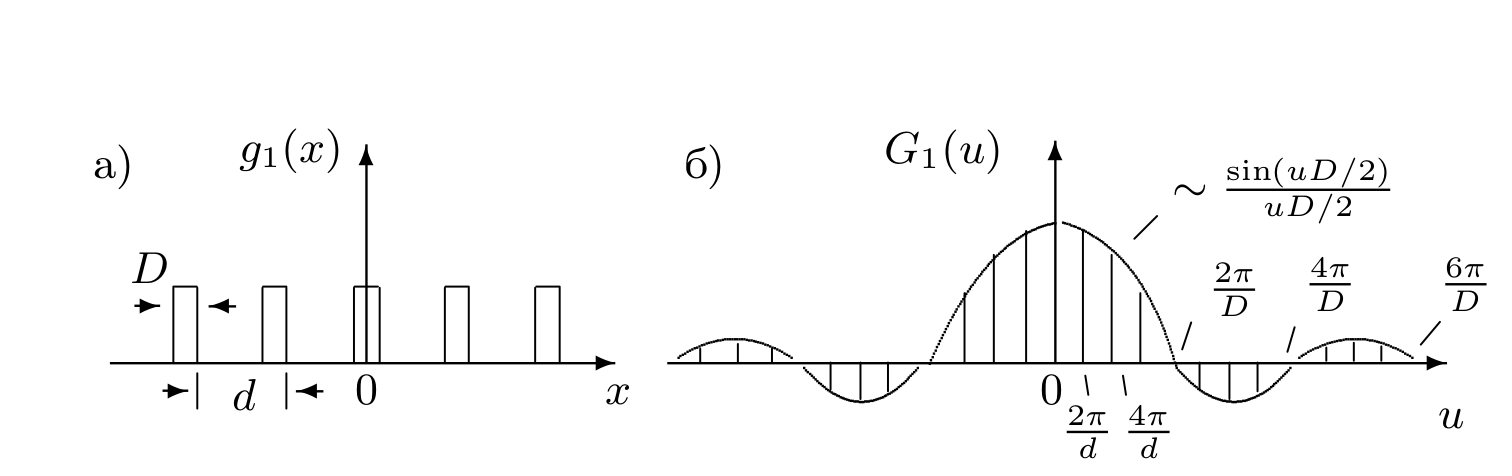
\includegraphics[width = 1.0\linewidth]{images/5.png}
	\caption{а) функция пропускания дифракционной решётки (последовательности прозрачных и непрозрачных полос);\\
б) $G_1 (u)$ "--- спектр функции пропускания дифракционной решётки}
\end{figure}	
Пространственное преобразование Фурье может осуществляться и в свободном пространстве при наблюдении дифракции Фраунгофера.
Если размеры дифракционной решётки неограничены, то дифракционные максимумы бесконечно узки. Чем меньше размер решётки (полное число щелей), тем шире каждый отдельный максимум.

Направление на главные максимумы $\theta_n = \frac{u n}{k} = \frac{\lambda n}{d}$ ($N$ "--- целое число) определяется приодом решётки d, а распределение амплитуд в спектре "--- фурье-образом функции пропускания отдельного штриха:
\[
g_2 (x) = \begin{cases} 1, & - \frac{D}{2} \leq x \leq \frac{D}{2} \\
						0, & - \frac{D}{2} > x > \frac{D}{2}
\end{cases}
\]
Вследсвие непереодичности $g_2(x)$, её фурье-образ представлятся непрерывным множеством точек и определяется интегралльным преобразованием Фурье:
\[
g(x) = \frac{1}{2 \pi} \int_{-\infty}^{+\infty} G(u) e^{iux} du,
\]
\[
G(u) = \int_{-\infty}^{+\infty} g(x) e^{-iux}dx.
\]
В таком виде $g(x)$ и $G(u)$ представляют собой пару преобразований Фурье: $G(u)$ "--- спектр или фурье-образ функци $g(x)$.
\[
	G_2 (u) = \int_{-\infty}^{+\infty} g_2 (x) e^{-iux} dx  = \int_{-D/2}^{+D/2} e^{-iux} dx = D \frac{\sin \frac{uD}{2}}{\frac{uD}{2}}.
\]
Введём понятие протяженности функции пропускания транспоранта ($\Delta x$) и ширины её спектра ($\Delta u$), тогда соотношение неопределённости принимает вид:
\[
	\Delta x \cdot \Delta u = \frac{2 \pi}{D} \cdot D = 2 \pi.
\]
Размер же малого объекта можно рассчитать, увеличив его изображение с помощью линзы.

\textbf{Метод Аббе}
Рассмотрим схему образования изображения. Пусть предмет расположен от линзы на большем расстоянии, чем фокусное, тогда существует сопряжённая предметной плоскости плоскость, где образуется изображение. Аббе предложил рассматривать схему прохождения в два этапа: сначала рассматривается первичное изображение (спектр в задней фокальной плоскости), затем это изображение рассматривается как источник волн, создающий изображение в другой плоскости (вторичное изображение). Этот подход опирается на принцип Гюйгенса-Френеля, согласно которому любой участок волнового фронта можно рассматривать как источник излучения. Под словами <<линза дважды осуществляет преобразование Фурье>> подразумевается следующее: сначала в задней фокальной плоскости линзы получается световое поле, соответствующее фурье-образу функции пропускания предмета (с точностью до фазы), а затем на промежутке между фокальной плоскостью и плоскостью изображения осуществляется обратное преобразование Фурье, в результате чего восстанавливается изображение предмета.

\textbf{Определение ширины щели с помощью линзы}
\begin{figure}[h!]
	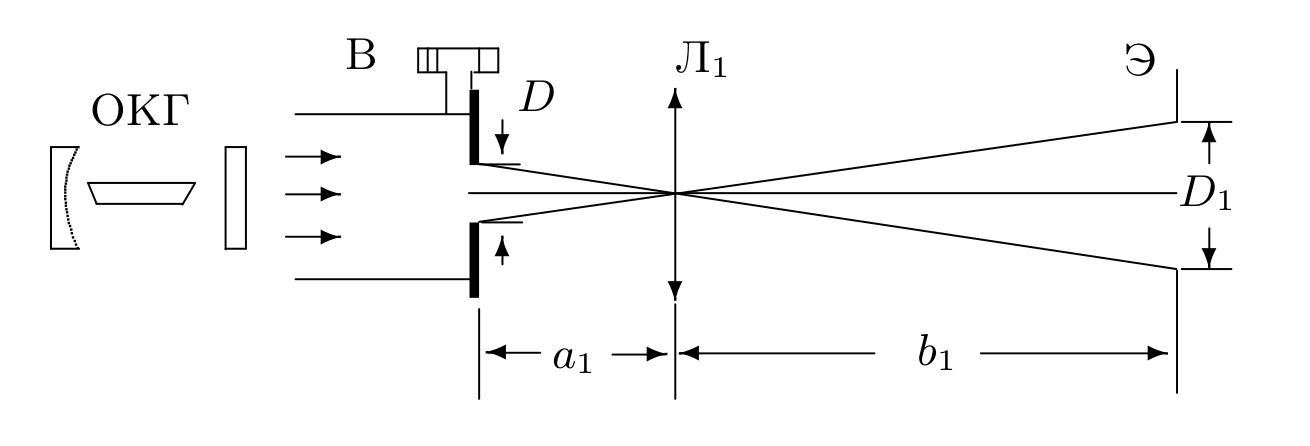
\includegraphics[width = 1.0\linewidth]{images/1.png}
	\caption{Схема для определения ширины щели с помощью линзы}
\end{figure}

\section*{Ход работы}

\subsection*{Определение ширины щели}

\subsubsection*{Определение ширины щели с помощтю линзы}

\begin{enumerate}

\item Соберем установку показанную на рис. 2 и включим в сеть блок питания лазера.

\item С помощью короткофокусной линзы $\text{Л}_1$ ($F = 38$ мм) получим на экране увеличенное изображение щели.

\item Меняя ширину щели от 50 до 500 мкм снимем зависимость размера изображения $D_1$ от ширины цели $D$. Данные запишем в таблицу:

\begin{center}
\begin{tabular}{|c|c|c|c|c|c|c|c|c|c|c|}
\hline 
$D,$ мкм & 50 & 100 & 150 & 200 & 250 & 300 & 350 & 400 & 450 & 500 \\ 
\hline 
$D_1,$ мм & 3 & 4 & 6 & 7 & 9 & 10 & 11 & 12 & 13 & 14 \\ 
\hline 
\end{tabular} 
\end{center}

Погрешности измерений:

\[\sigma_D = 5 \: \text{мкм} \quad \sigma_{D_1} = 0,5 \text{мм}\]

\item По ихмеренным данным построим график зависимость $D_1 (D)$:

\begin{figure}[h!]
	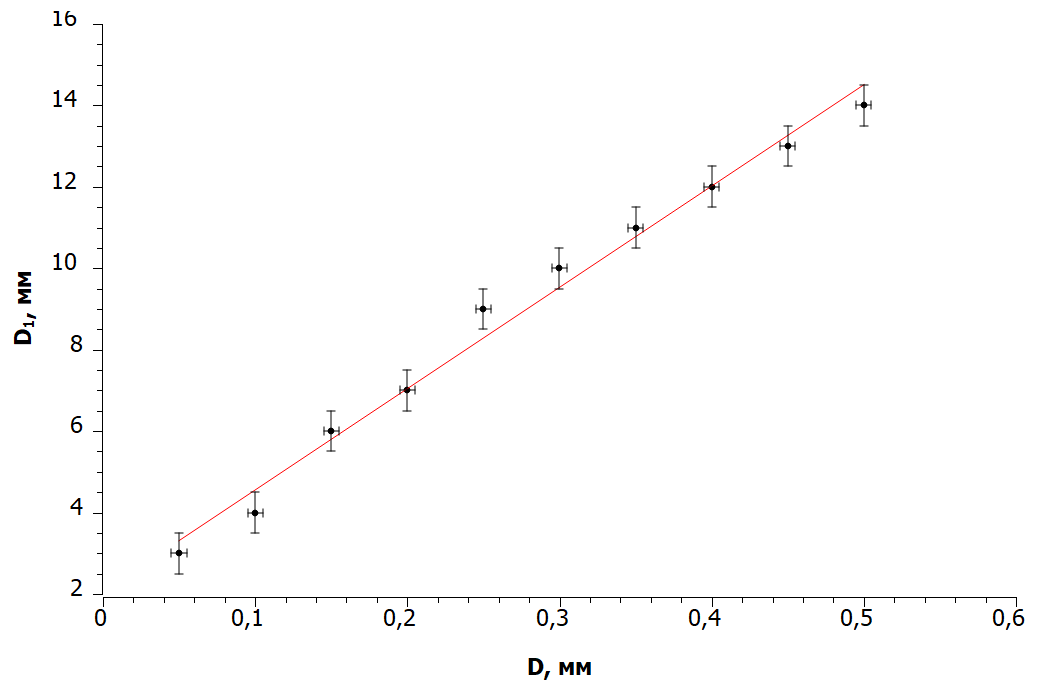
\includegraphics[width = 1.0\linewidth]{images/graph_1.png}
	\caption{График зависимости размера изображения от ширины щели}
\end{figure}

Получим зависимость вида $y = ax + b$ - $a = 24,8 \pm 1,0$, $b = 2,07 \pm 0,30$. Следовательно:

\[\text{Г} = \frac{D_1}{D} = a = 24,8 \pm 1,0\]

\item Измерим расстояния $a_1$ и $b_1$:

\[a_1= 40\pm 1 \: \text{мм} \quad b_1 = 1080 \pm 1 \: \text{мм}\]

По ним получим:

\[\text{Г} = \frac{b_1}{a_1} = 27,0 \pm 0,7\]

\item Видим, что полученные значения немного отличаются, это может быть связано с неточностью определения ширины щели из-за люфта микрометра.

\end{enumerate}

\subsubsection*{Определение ширины цели по ее спектру}

\begin{enumerate}

\item Соберем схему показанную на рис. 4.

\begin{figure}[h!]
	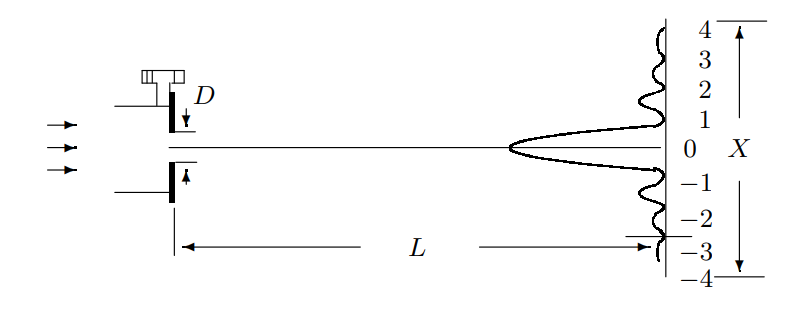
\includegraphics[width = 1.0\linewidth]{images/6.png}
	\caption{Схема для определения ширины щели по спектру}
\end{figure}

\item Проведем серию измерений $X(m)$, где $m$ - порядок минимума, меняя ширину щели. Запишем данные в таблицу:

\begin{center}
\begin{tabular}{|c|c|c|c|c|c|c|c|c|c|c|}
\hline 
$X,$ мм & 145 & 132 & 110 & 97 & 108 & 99 & 90 & 108 & 85 & 77 \\ 
\hline 
m & 2 & 4 & 5 & 6 & 8 & 8 & 9 & 13 & 11 & 11 \\ 
\hline 
$D,$ мкм & 30 & 50 & 70 & 90 & 100 & 120 & 140 & 100 & 180 & 200 \\ 
\hline 
\end{tabular} 
\end{center}

Погрешности измерений:

\[\sigma_X = 1 \: \text{мм} \quad \sigma_D = 5 \: \text{мкм} \]

\item По результатам измерения спектра рассчитаем ширину щели $D_c$ (<<c>> - по спектру) используя соотношения:

$\bigtriangleup X = \frac{X}{2m} = \frac{\lambda}{D_c} L,$

где $\lambda = 632,8$ нм. Построим на одном листе графики $D_{\text{л}} = f(D)$ (<<л>> - по линзе) и $D_c = f(D)$:

\begin{figure}[h!]
	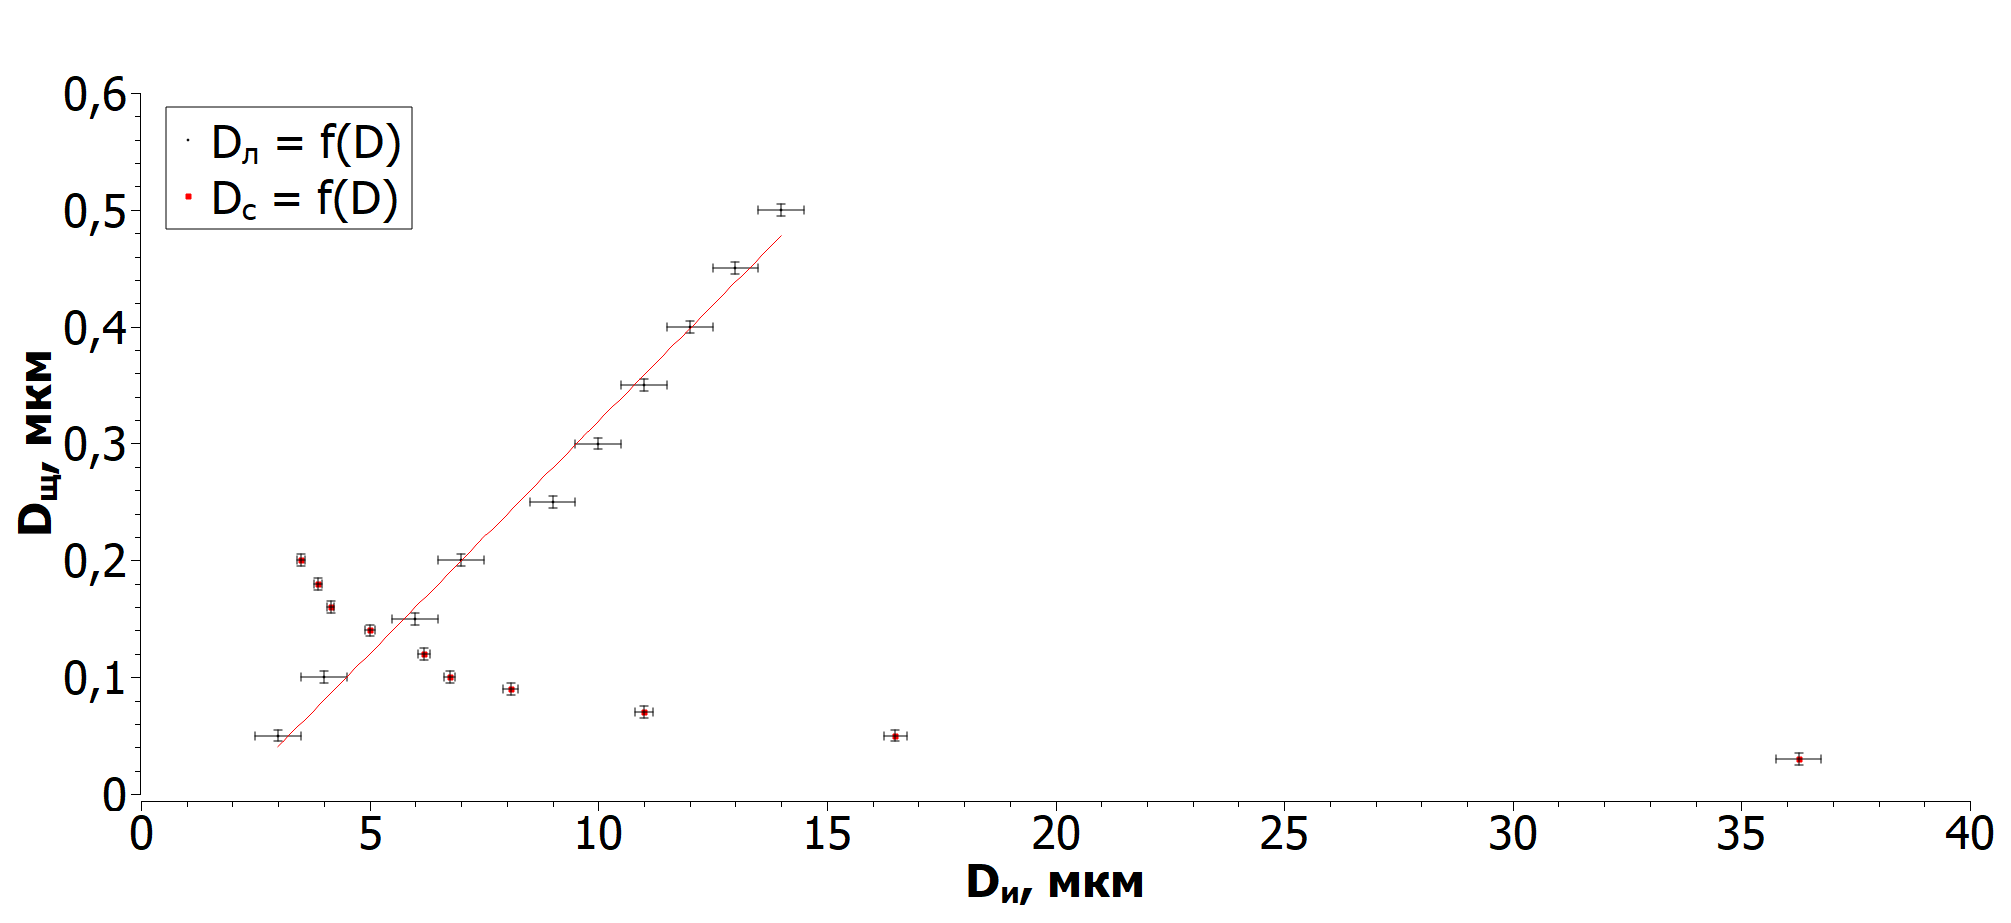
\includegraphics[width = 1.0\linewidth]{images/graph_3.png}
	\caption{$D_{\text{л}} = f(D)$ и $D_c = f(D)$}
\end{figure}

\end{enumerate}

\newpage

\subsection*{Определение периода решеток}

\subsubsection*{Определение периода по спектру на удаленном экране}

\begin{enumerate}

\item Поставим каасету с двумерными сетками вплотную к выходному окну лазера. Для каждой сетки измерим расстояние X, между m-ми максимумами и отметим m = порядок максимума (получившуюся картину можно наблюдать на рис. 6). Запишем полученные данные в таблицу:

\begin{center}
\begin{tabular}{|c|c|c|c|c|c|}
\hline 
№ & 1 & 2 & 3 & 4 & 5 \\ 
\hline 
$m$ & 3 & 4 & 4 & 5 & 8 \\ 
\hline 
$X_m,$ мм & 217 & 192 & 96 & 60 & 78 \\ 
\hline 
\end{tabular} 
\end{center}

Погрешность измерения $X_m$ составила:

\[\sigma_{X_m} = 1 \: \text{мм}\]

\begin{figure}[h!]
    \centering
	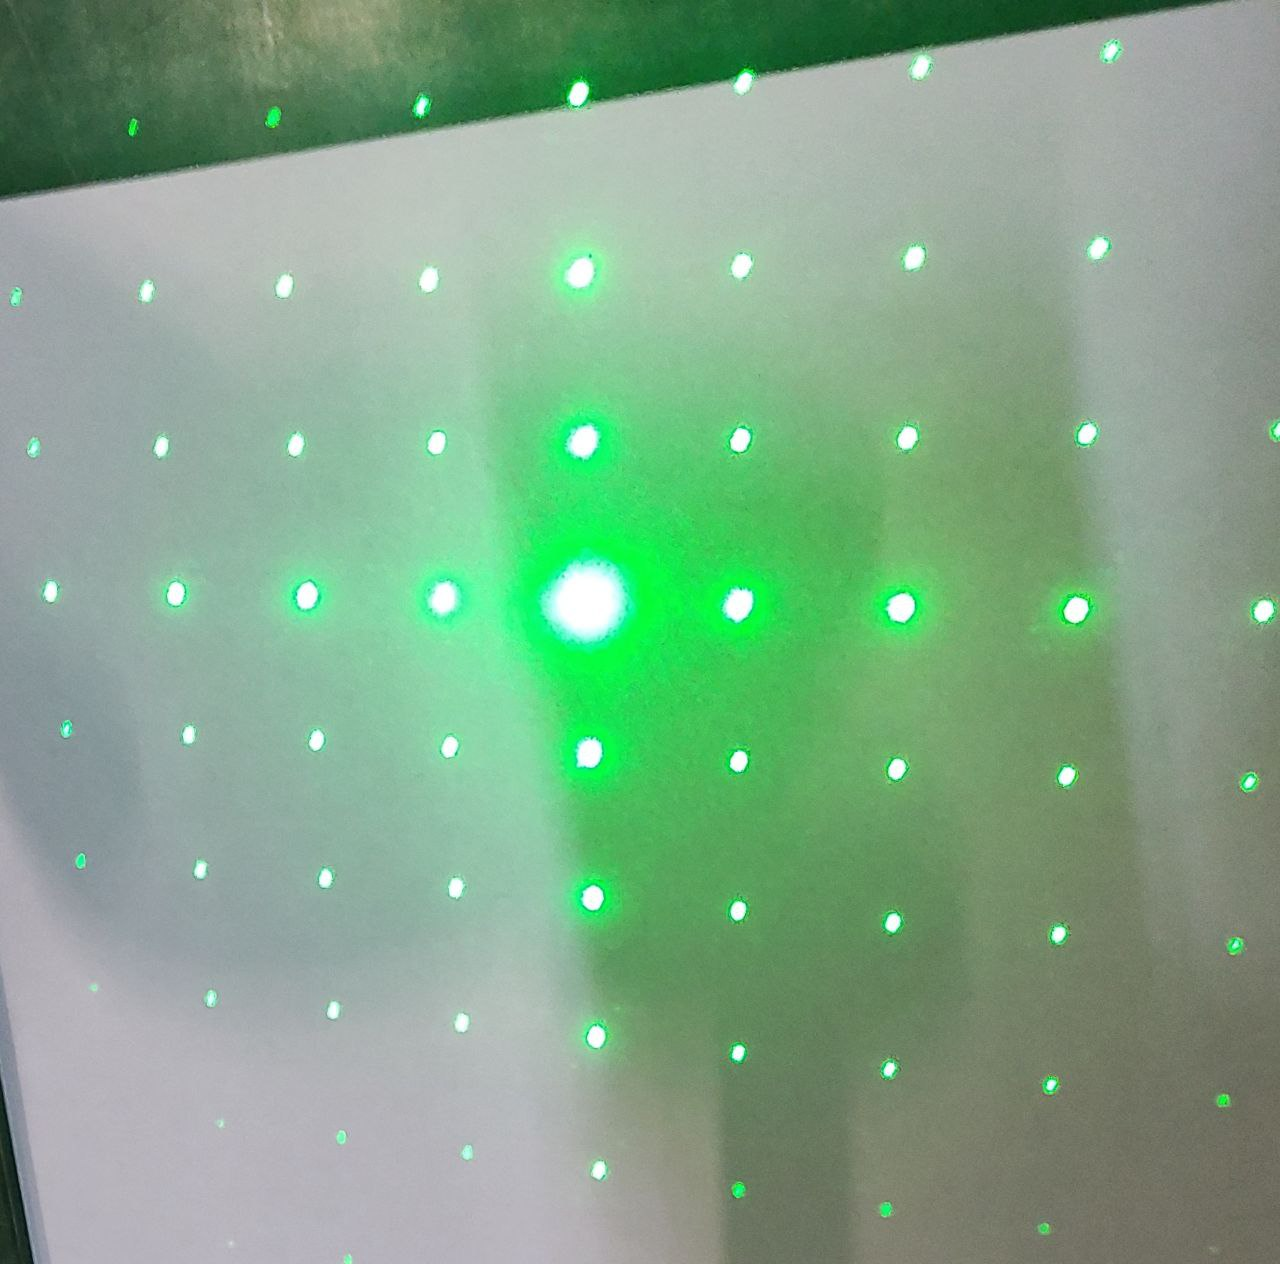
\includegraphics[width = 0.5\linewidth]{images/img_1.jpg}
	\caption{Картина получившаяся для решетки с номером 2}
\end{figure}

\item Рассчитаем расстояния $\bigtriangleup X$ для каждой решетки между соседними максимумами и определим период каждой решетки $d_c = f(№)$ используя соотношение:

\begin{equation}
\bigtriangleup X = \frac{X}{2m} = \frac{\lambda}{d_c} L,
\end{equation}

где L - расстояние от кассеты до экрана и $L = 132,0 \pm 0,1$ см. Запишем полученнные данные в таблицу:

\begin{center}
\begin{tabular}{|c|c|c|c|c|}
\hline 
№ & $\bigtriangleup X,$ мм & $\sigma_{\bigtriangleup X},$ мм & $d_c$, мкм & $\sigma_{d_c},$ мкм \\ 
\hline 
1 & 72,3 & 0,3 & 11,5 & 0,1 \\ 
\hline 
2 & 48,0 & 0,3 & 17,4 & 0,1 \\ 
\hline 
3 & 24,0 & 0,3 & 34,8 & 0,4\\ 
\hline 
4 & 12,0 & 0,2 & 69,6 & 1,2\\ 
\hline 
5 & 9,8 & 0,1 & 85,7 & 1,1 \\ 
\hline 
\end{tabular} 
\end{center}

\end{enumerate}

\subsubsection*{Определение периода решеток по увеличенному изображению спектра}

\begin{enumerate}

\item Соберем схему показанную на рис. 7. Линзу $\text{Л}_2$ с максимальным фокусом ($F_2 \simeq 10$ см) поставим на расстоянии $\simeq F_2$ от кассеты. В плоскости Ф линза $\text{Л}_2$ дает фрье-образ сетки - её спектр, а короткофокусная длинза $\text{Л}_3$ ($F_3 \simeq 2,5$ см) создаёт на экране увеличенное изображение этого спектра.

\begin{figure}[h!]
    \centering
	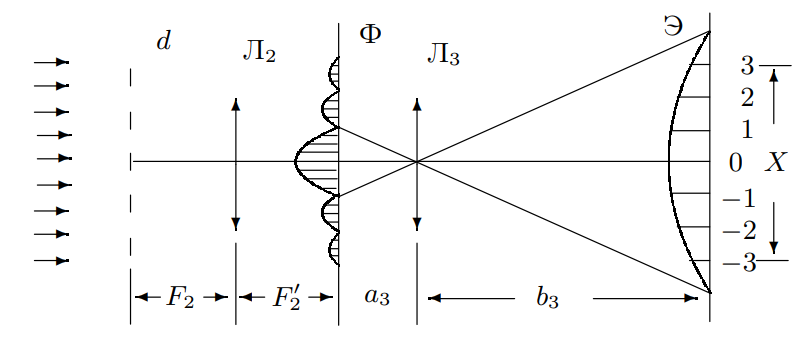
\includegraphics[width = 0.8\linewidth]{images/7.png}
	\caption{Схема определения периода решетки по увеличенному изображению спектра}
\end{figure}

\item Измерим X и m для всех сеток, где это возможно. Запишем данные в таблицу:

\begin{center}
\begin{tabular}{|c|c|c|c|c|}
\hline 
№ & 2 & 3 & 4 & 5 \\ 
\hline 
$m$ & 1 & 2 & 4 & 5 \\ 
\hline 
$X_m,$ мм  & 192 & 190 & 192 & 178 \\ 
\hline 
\end{tabular} 
\end{center}

Погрешность измерения $X_m$ составила:

\[\sigma_{X_m} = 1 \: \text{мм}\]

\item Запишем чему равно $a_3$, $b_3$, $F_2$ и $F_3$:

\[F_2 = 110 \: \text{мм} \quad F_3 = 25 \: \text{мм}\]

\[a_3 = 25 \pm 1 \: \text{мм} \quad b_3 = 1080 \: \text{мм}\]

\item Зная увеличение линзы $\text{Л}_3$ ($\text{Г}_3 = b_3 / a_3$), можно расссчитать расстояние между максимумами $\bigtriangleup x$ в плоскости Ф, а затем период сетки $d_{\text{л}}$ по формуле:

\begin{equation}
\bigtriangleup x = \frac{\bigtriangleup X}{\text{Г}_3} = \frac{\lambda}{d_{\text{л}}} F_2
\end{equation}

\item Рассчитаем нужные значения и запишем их в таблицу:

\begin{center}
\begin{tabular}{|c|c|c|c|c|}
\hline 
№ & $\bigtriangleup x,$ мм & $\sigma_{\bigtriangleup x},$ мм & $d_{\text{л}},$ мкм & $\sigma_{d_{\text{л}}},$ мкм \\ 
\hline 
2 & 4,44 & 0,18 & 15,7 & 0,6 \\ 
\hline 
3 & 2,20 & 0,09 & 31,7 & 1,3 \\ 
\hline 
4 & 1,11 & 0,04 & 62,6 & 2,5 \\ 
\hline 
5 & 0,82 & 0,03 & 84,5 & 3,4 \\ 
\hline 
\end{tabular} 
\end{center}

\end{enumerate}

\subsection*{Мультиплицирование}

\begin{enumerate}

\item Снова поставим тубус со щелью к окну лазера (рис. 8) и найдем на экране резкое изображение щели с помощью линзы $\text{Л}_2$ ($F_2 = 110,$ мм). В фокальной плоскости линзы поставим кассету с сетками.

\begin{figure}[h!]
    \centering
	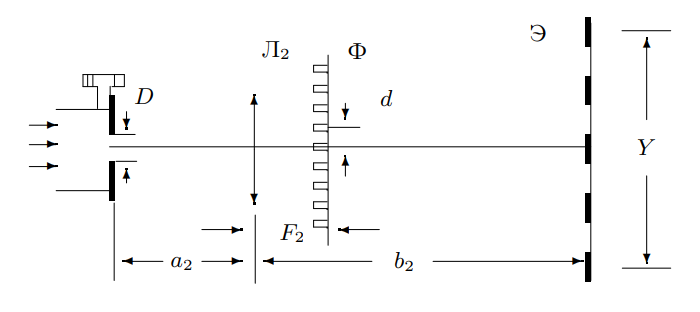
\includegraphics[width = 0.8\linewidth]{images/8.png}
	\caption{Схема для наблюдения мультиплицирования}
\end{figure}

\item Подберем такую ширину входной щели $D$, чтобы на экране можно было наблюдать мультиплицированное изображение для всех сеток ($D = 80 \pm 5,$ мкм). Измерим расстояния $a_2$ и $b_2$:

\[a_2 = 140 \pm 1 \: \text{мм} \quad b_2 = 1100 \pm 1 \: \text{мм}\]

\item Снимем зависимость $Y$ (расстояние между удаленными изображениями щели) и $K$ (число промежутков между изображениями) от № (номера сетки):

\begin{center}
\begin{tabular}{|c|c|c|c|c|c|}
\hline 
№ & 1 & 2 & 3 & 4 & 5 \\ 
\hline 
$Y,$ мм & 171 & 151 & 71 & 65 & 50 \\ 
\hline 
$K$ & 3 & 4 & 4 & 7 & 7 \\ 
\hline 
\end{tabular} 
\end{center}

\item Рассчитаем периоды <<фиктивных>> решёток. которые дали бы такую же периодичность на экране: $\bigtriangleup y = \bigtriangleup Y / \text{Г}_2$, где $\bigtriangleup Y = Y/K$. Также рассчитаем $d_c$ - периоды решёток, определенных по спектру. Зависимость должна быть линейной, поскольку:

\[\frac{\lambda}{\bigtriangleup y} F_2 = d_c\]

Запишем результаты расчетов в таблицу:

\begin{center}
\begin{tabular}{|c|c|c|c|c|}
\hline 
№ & $\bigtriangleup y$, мм & $\sigma_{\bigtriangleup y},$ мм & $1/d_c,$ 1/мкм & $\sigma_{1/d_c},$ 1/мкм \\ 
\hline 
1 & 7,25 & 0,05 & 0,0866 & 0,0004 \\ 
\hline 
2 & 4,80 & 0,03 & 0,0575 & 0,0003 \\ 
\hline 
3 & 2,26 & 0,02 & 0,0287 & 0,0003 \\ 
\hline 
4 & 1,18 & 0,01 & 0,0144 & 0,0002 \\ 
\hline 
5 & 0,91 & 0,01 & 0,0117 & 0,0001 \\ 
\hline 
\end{tabular} 
\end{center}

\item Построим график зависимости $\bigtriangleup y = f(1/d_c)$.

\begin{figure}[h!]
    \centering
	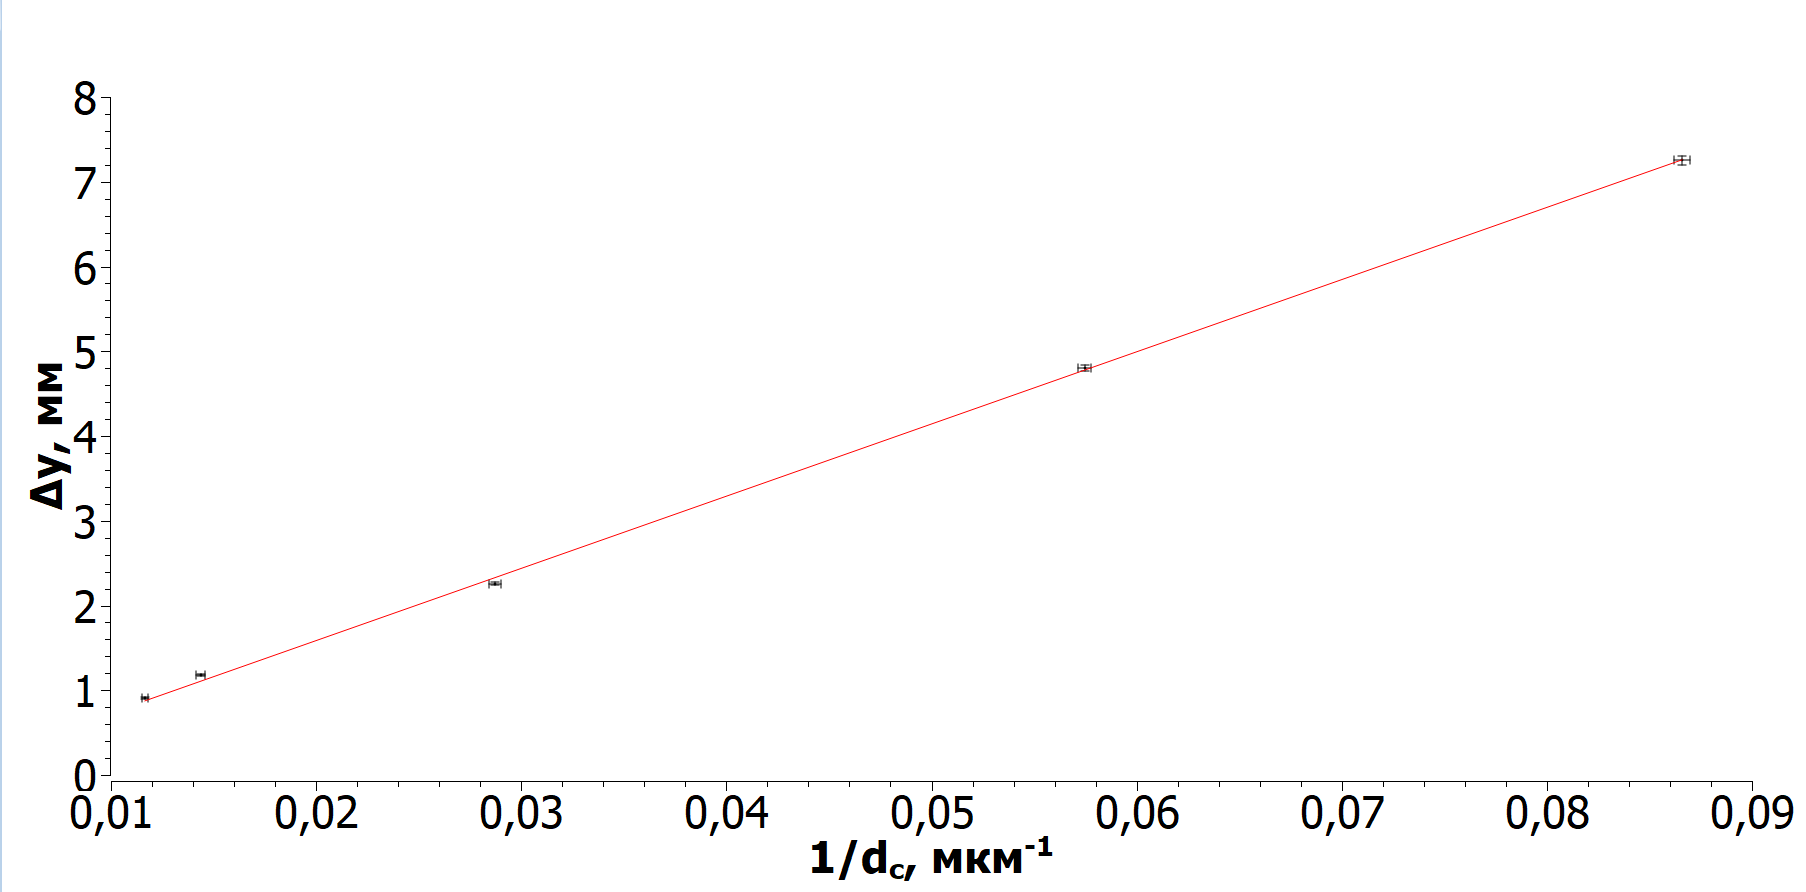
\includegraphics[width = 0.8\linewidth]{images/graph_4.png}
	\caption{График зависимости $\bigtriangleup y = f(1/d_c)$}
\end{figure}

Зависимость имеет вид $y = ax + b$, где:

\[a = (85,2 \pm 0,2) \cdot 10^3 \: \text{мкм}^2 \quad b = -0,117 \pm 0,017 \: \text{мм}\]

\end{enumerate}

\subsection*{Влияние щелевой диафрагмы на изображение сетки}

\begin{enumerate}

\item Вертикальная и горизонтальная щели. 1 спектр - картина не разрешается, 2 и более, картина разрешается.

\begin{figure}[h!]
        \begin{center}
            \begin{minipage}[h!]{0.48\linewidth}
                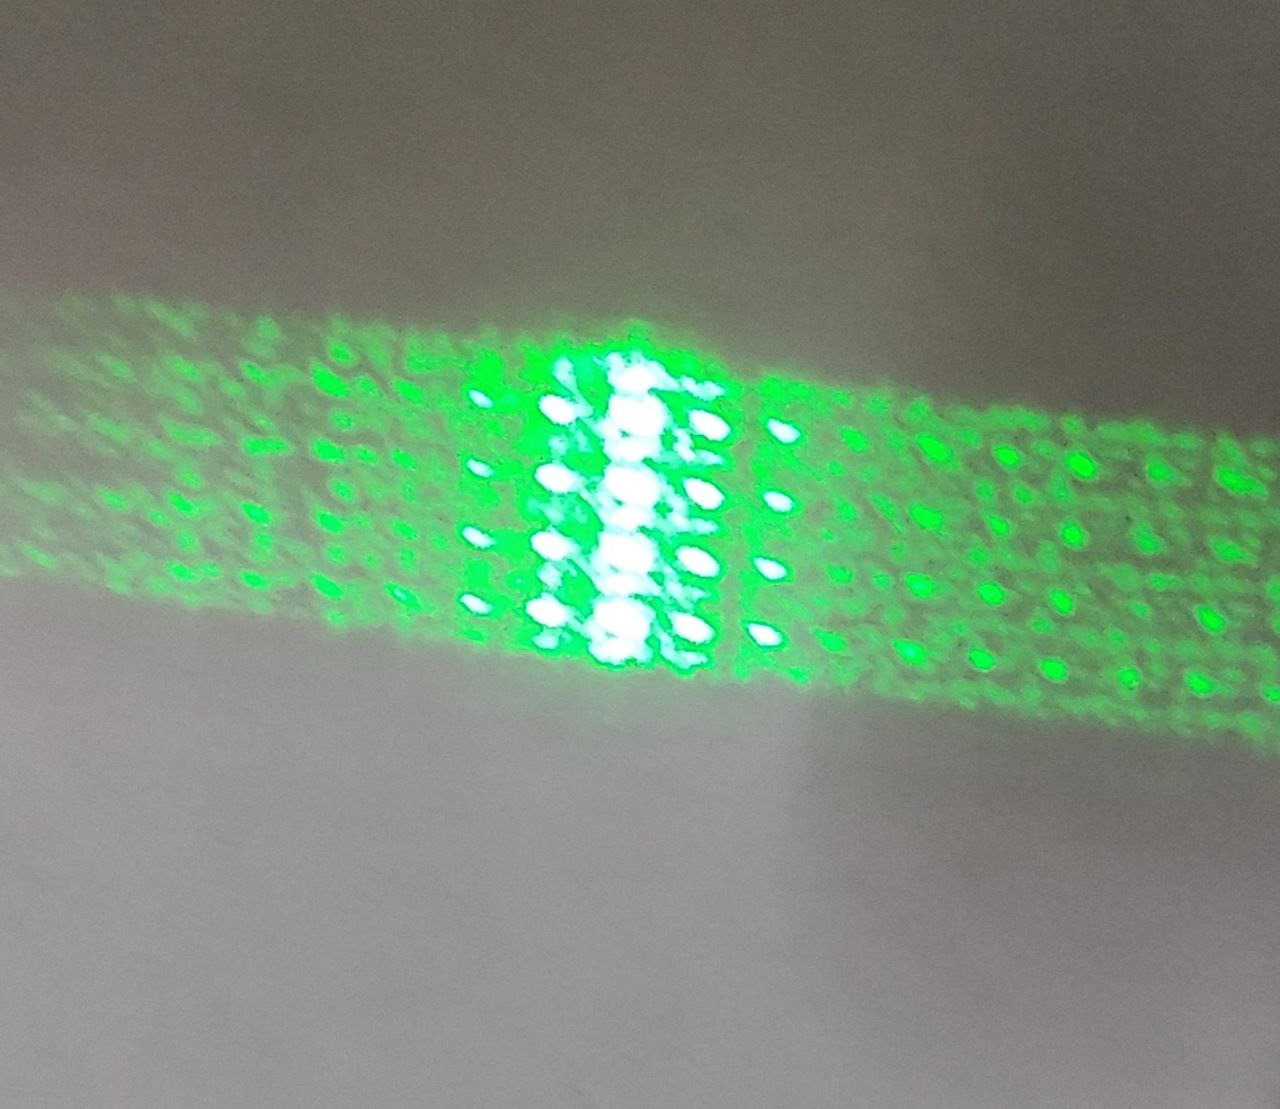
\includegraphics[width=1\linewidth]{images/img_3.jpg}
                \caption{Изображение щели на экране}
                \label{picture_2}
            \end{minipage}
            \hfill
            \begin{minipage}[h!]{0.48\linewidth}
                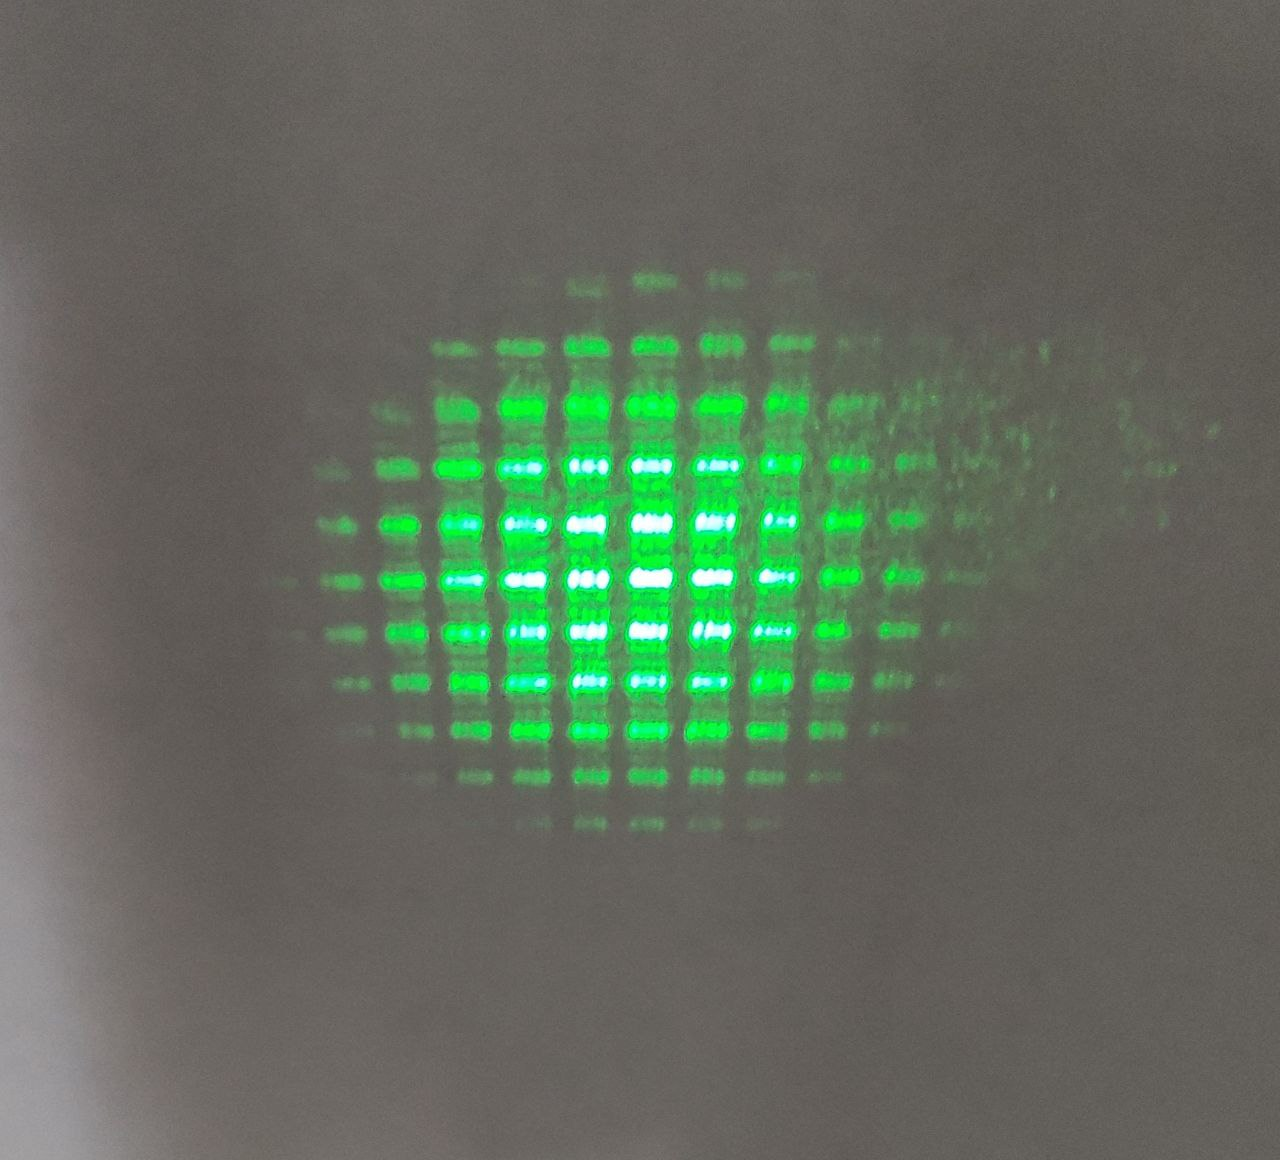
\includegraphics[width=1\linewidth]{images/img_2.jpg}
                \caption{Увеличенное изображение спектра}
                \label{picture_3}
            \end{minipage}
        \end{center}
    \end{figure}
    
    \begin{figure}[h!]
        \begin{center}
            \begin{minipage}[h!]{0.48\linewidth}
                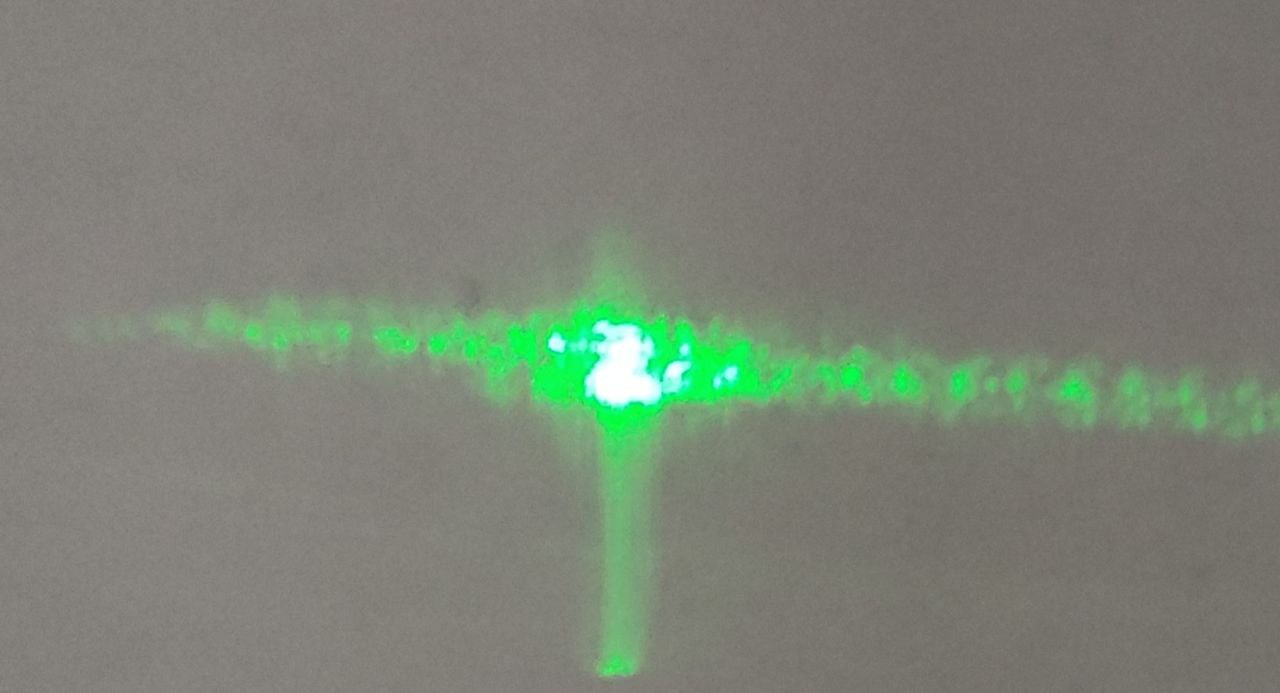
\includegraphics[width=1\linewidth]{images/img_5.jpg}
                \caption{Изображение узкой щели на экране}
                \label{picture_2}
            \end{minipage}
            \hfill
            \begin{minipage}[h!]{0.48\linewidth}
                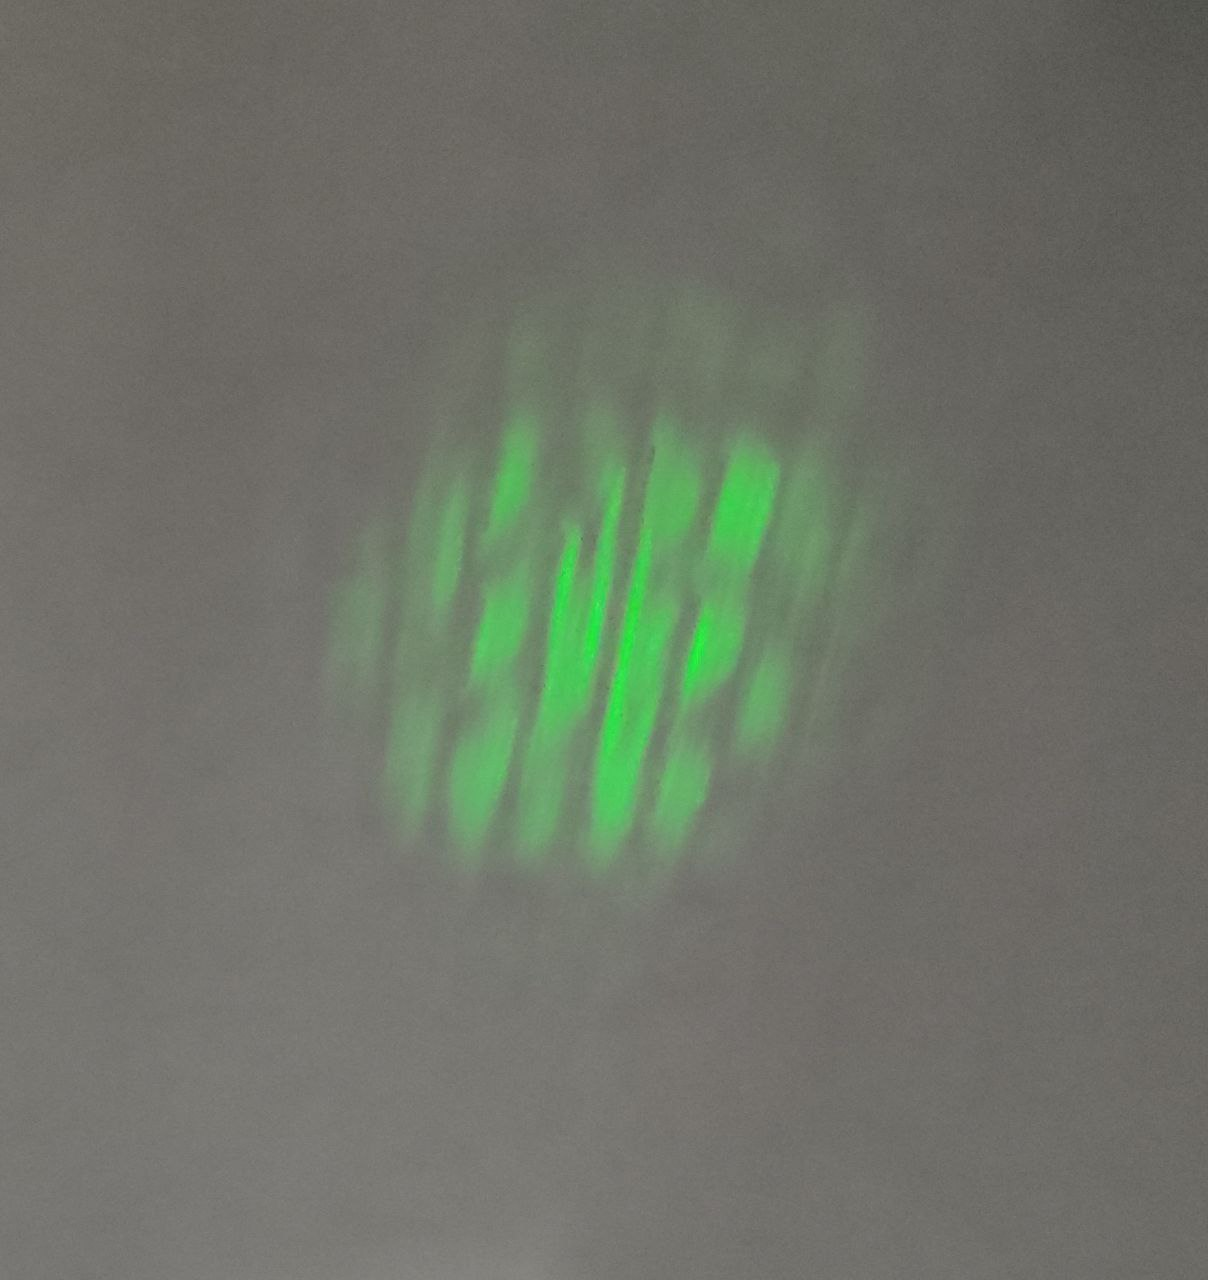
\includegraphics[width=1\linewidth]{images/img_4.jpg}
                \caption{Увеличенное изображение спектра для узкой щели}
                \label{picture_3}
            \end{minipage}
        \end{center}
    \end{figure}

\item Щель под углом в $45^{\circ}$. 2 спектра - картина не разрешается,3 и более разрешается.

\end{enumerate}

\section*{Вывод}

Мы научились исследовать параметры паттернов через порождающие дифракционные
картины с помощью разложения в ряд фурье. В частности мы происследовали поведение
щели и двумерных решеток. В экспериментах мы получили различные числовые значения, подтверждающие друг друга.


\end{document}